\pdfoutput=1

\documentclass{l4proj}
\usepackage{comment}
\usepackage{graphicx}
\usepackage{caption}
%
% put any packages here
%


\begin{document}
\title{Designing a lightweight protocol for constrained devices for use in the Internet of Things paradigm}
\author{Fergus Leahy}
\date{\today}
\maketitle

\begin{abstract}
\textbf{PLACEHOLDER}
A level 4 project which explores the current use of protocols for the Internet of things devices.
\end{abstract}

\educationalconsent
%
%NOTE: if you include the educationalconsent (above) and your project is graded an A then
%      it may be entered in the CS Hall of Fame
%
\tableofcontents
%==============================================================================

\chapter{Introduction}
\pagenumbering{arabic}

The ``Internet of Things'' paradigm along with the ``Smart'' prefix has recently seen a significant rise in interest and popularity with manufacturers, hobbyists and end-users. Everything from your set-top box to your washing machine can now be ``Smart'' and connect to the Internet to tell you if your favourite TV show has downloaded or that your wash cycle has complete\cite{LG, SmartCraze}. Some hobbyists have gone so far to make a plant send a text or tweet when it needs watering\cite{Botanicalls, TweetPlant}.

This uptake in interest and development can be largely attributed to the advent of lower power, smaller and cheaper devices. Large companies, such as the mobile phone chip-set manufacturer, Qualcomm, recently declared their support at CES 2012 with the announcement of a dedicated development platform for the ``Internet of Things''\cite{Qualcomm}.

Similarly there has also been much enthusiasm from small companies and start-ups trying to create the next hit consumer device. Social funding platform, Kickstarter\cite{Kickstarter}, has seen many attempts at creating the perfect ``Thing'' for the Internet\cite{SmartThings, Twine}.

Whilst all of these devices from manufacturers, start-ups and hobbyists may very well be great ``Things'' by themselves, there exists a problem. How does one connect all of these heterogeneous platforms and devices together to create a true interconnected ``Internet of Things''?

This project focuses on just that and endeavours to create a communication protocol that is not only platform agnostic but also lightweight enough to be run on the most constrained devices, such as the TelosB Sky Motes(8MHz CPU,10K ram)\cite{TelosB}. Another core design focus is that the protocol must be able to scale effectively as the network dramatically increases size as can be expected with the rapidly increasing availability of network-connected devices.

%==============================================================================

\chapter{Background and Related Work} % (fold)
\label{cha:background}

\section{Internet of Things paradigm} % (fold)
\label{sec:internet_of_things_paradigm}


The standard model of how we use computers and the Internet today revolves around the idea of an interconnected network of servers, routers and data centres around which users connect using their personal computers to access, input, manipulate and retrieve data. 

This model heavily relies upon the users to provide the data from which the Internet is powered. Without this data the Internet would be a barren place, with nothing to search for, sell, buy, share, watch, listen to, play, analyse or learn from.
Users from all around the world have contributed to make the Internet \textit{the} single biggest resource in the world by snapping photos, capturing videos, writing blogs, creating websites, commenting, discussing, reviewing, buying, selling and inputting data. So much data in fact that the estimated size of the Internet in 2009 was 500bn gigabytes, of which 70\% was contributed to by users.\cite{Size}   

% INSERT DIAGRAM HERE
Within this model there exists two significant problems posed by users; time and accuracy. In terms of time, users only have so many hours in a day to input data; which can only be so accurate as all users are prone to error through one means or another.
These two problems make it difficult to observe our world and represent it in an accurate and reliable digital form.

The idea of taking this responsibility of inputting data away from the user and giving it to the machine is where the ``Internet of Things'' term initially came from. The term itself was thought to have first been coined by Kevin Ashton\cite{K.Ashton} in 1999, who at the time was interested in linking up a company's supply chain to the Internet using RFID technology to allow for autonomously monitoring its state.
Sadly at that time the idea progressed little and didn't garner much support.

Fast forward to 2013, the ``Year of the Internet of Things'' as declared by the MIT Technology Review\cite{2013IoT} and observed in the Consumer Electronics Show 2013 (CES) with manufacturers introducing everything from smart fridges to smart washing machines. Parallel to this, low power devices have become increasingly affordable and small enough to embed into other devices making it much more possible to create a truly autonomous system, either in the home, office or car, wherein the user doesn't have to interact directly with any of the devices but instead just go about daily life, which, in the background is enhanced by these ubiquitous devices operating together.

With all the possible ``Things'' that can exist, the core functionality in the ``Internet of Things'' can be simply modelled as closed loop system in which it can sense, process and interact with the real world as well as other devices and services. This system is represented at its simplest by an if statement, \textit{if \textbf{event occurs} then \textbf{do action}}, which provides developers and users alike an easy to understand yet powerful model to create rules for autonomous interaction.i.e.
\begin{center}
	\textit{if \textbf{temp \textless  20C} then \textbf{Turn ON heating}}

	\textit{if \textbf{washing machine done} then \textbf{Text John}}
\end{center}

There currently exists a variety of online services and devices which give the end-user this ability to do such tasks, such as the Twine device \cite{Twine} which is a small low power device with a variety of sensors and a WI-FI radio. The goal of the device was to make it simple and easy to set up and use; the user just puts the device in the desired environment, perhaps on a washing machine, sets up some rules such as ``When accelerometer is knocked Then tweet''. When the condition is true, the preset action, in this case tweeting, is performed. Whilst this gives the user great flexibility to perform actions automatically, the limitations show when trying to interact with more than one Twine or with other devices and not just Internet services. 

\begin{figure}[h]
	\centering
	\begin{minipage}{.5\textwidth}
		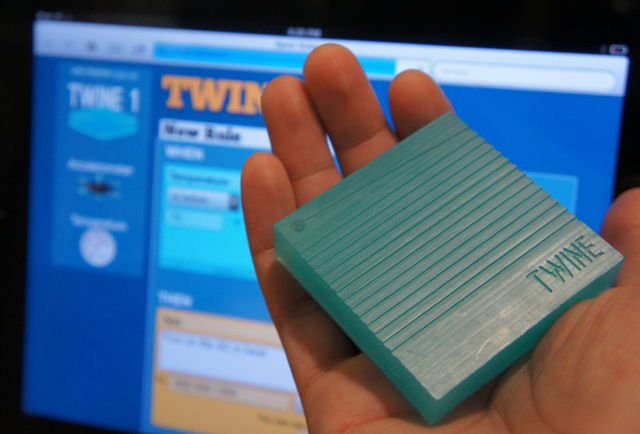
\includegraphics[width=.6\linewidth]{twine-device.jpg}
		\captionof{figure}{Twine IoT device.}
		\label{fig:twine_device}
	\end{minipage}%
	\begin{minipage}{.5\textwidth}
		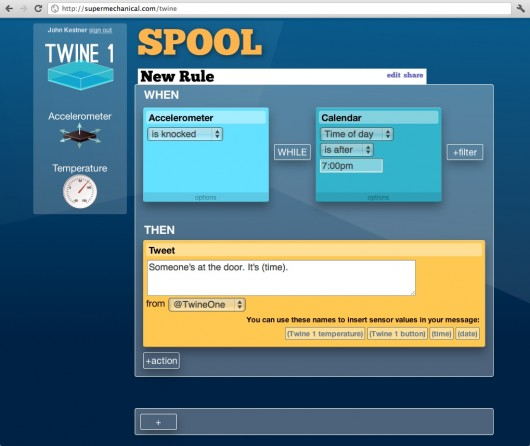
\includegraphics[width=.6\linewidth]{twine-rules.jpg}
		\captionof{figure}{Twine rule, When x Then y}
	\end{minipage}
\end{figure}

The Twine device isn't the only device out there, Smart Things\cite{SmartThings} goes one step further than Twine and gives the user a network of devices connected to the Internet through a central hub which the user can then interact with online.

The main problem that exists and will continue to be so is that the digital environment is filled with a huge variety of heterogeneous devices. The key to the future of the ``Internet of Things'' is to find a way to abstract the differences between these devices and create a simple platform on which all types of devices can communicate to build a more rich and powerful ``Internet of Things''.

 % Kevin Ashton, RFID, coined IoT
 % http://www.rfidjournal.com/article/view/4986
 % Giving everyday objects a digital presence and creating machine to machine connections
 % Autonomy, semi-autonomy
 % Taking the human out of the equation and empowering the computer to produce and consume its own data to make our world more 
 % efficient, less wasteful, more time and less energy.
 % Slow start, not much going on.

 % 2012/13 jump start, lots of manufacturers
 % open hardware initiatives
 % linking home automation, security and IoT i.e. toaster/coffee machine
 % 

 %%%%%%%%%%%%%%%%%%%%%%%%%%%%%%%%%%%%%%%%%%%%%%
% HOME AUTOMATION? ??????????????????????
%%%%%%%%%%%%%%%%%%%%%%%%%%%%%%%%%%%%%%%%%%%%%%%%%%


% section internet_of_things_paradigm (end)
\newpage
\section{Open source constrained devices} % (fold)
\label{sec:open_source_constrained_devices}

In the past 5-10 years, there have been many attempts at creating an affordable, low power and approachable electronics platform such as Arduino, Netduino, BeagleBone, Teensy and MSP430 Launchpad. All of which have taken very different approaches, some opting for absolute low cost (MSP430 Launchpad), whilst others aimed to be fully featured and powerful devices (BeagleBone). Other devices such as the TelosB mote, whilst not cheap, has fuelled academic research into new ways of designing and implementing Wireless Sensor Networks. More recently, the Raspberry Pi has created a whole new market of super, low-cost, yet moderately-powerful computers aimed at education and hobbyists.

In the rest of this section a variety of different devices and platforms will be discussed including the Arduino, TelosB mote, Raspberry Pi and other ``Internet of Things'' related devices. 

\subsection{Arduino} % (fold)
\label{sub:arduino}

The Arduino was born in 2005 at an Italian university, Interaction Design Institute Ivrea, out of the necessity of creating a cheap and approachable electronics platform which could enable design students to create interaction design projects without the need of an electronics background.
The main device which was created and has remained much the same since, is based on an Amtel ATmega328 8bit micro-controller running at 16MHz with 2KB of RAM and 32KB of storage for programmes written in a variation of C/C++. The board itself maps out the micro-controller's mix of 20 digital and analogue input/output pins and supports several standardised protocols for communicating with other devices such as I\textsuperscript{2}C\footnote{I\textsuperscript{2}C - Inter-Integrated Circuit} and UART\footnote{UART - Universal Asynchronous Reciever/Transmitter}. 

But the key to the Arduino Platform is not the micro-controller itself but instead the design, software and support provided by the creators and other developers. The other major factor to its success is that the device, along with the documentation and support, are all open source, thus allowing anyone to learn from, replicate and expand upon the platform in any way they wish.

An example of how these factors have had a hugely positive effect is something which Arduino calls ``Shields''. These shields plug in on top of the Arduino board and contain standard components which can add additional features such as WI-FI, Ethernet, sound, motor control etc. Rather than users being required to find, purchase and solder the required components to add such features, these pre-built shields provide it in simple and readily available package, made by a variety of manufacturers.

Since its creation, the Arduino platform has created a range of Arduino named devices and shields resulting in a following of over 300,000 users\cite{ArduinoNumbers} and support from many manufacturers and distributors worldwide. 

Due to Arduino's open policy many new start-ups have been able to quickly design prototypes and products using the Arduino platform which have been taken to market in various refined forms. Often the same micro-controller which powers the Arduino is kept and the board miniaturised to fit the product's needs. Products such as the Internet ``Thing'' Twine\cite{Twine} and the Smart Things ``Internet of Things'' eco-system have taken this approach\cite{SmartThings}.

However, whilst there is an abundance of Arduino devices in the wild with many being used as an Internet ``Thing'', there is yet to be created an open and compatible method to easily network a group of such devices together to form a connected ``Internet of Things'' network.

\begin{comment}
OPEN SOURCE
Micro-controller, cheap, easy, PIC chips were difficult, lowered barrier of entry, provided large support and huge following
Italian made, several iterations on size and power
Good starting point for development as there are many in existence
Well adopted
Based on C/C++ with a few tweaks, offers shields for expandability i.e. Ethernet, WI-FI
very good at sensing and doing things
16MHz
no threading
\end{comment}
% subsection Arduino (end)

\newpage
\subsection{Raspberry Pi} % (fold)
\label{sub:raspberry_pi}
Launched in 2012 the Raspberry Pi, a \$35 credit card sized computer, was eagerly anticipated to change the computing landscape. The charity behind it, the Raspberry Pi foundation, had one main goal; to refresh and promote the teaching of computer science in schools.

Similar to the Arduino Platform, most of the hardware and software for the device is open source with the aim of letting adults and children alike get their hands dirty learning about computing without the worry of breaking an expensive computer.

The Raspberry Pi itself is a moderately well powered, single-board computer capable of running a wide variety of Linux-based operating systems. It's host to a 700MHz ARM CPU, 512MB RAM and a variety of inputs/outputs including an Ethernet port. These features, along with some additional GPIO\footnote{General Purpose Input Output} pins, just like the Arduino, allow it to sense and control the world around it, thus making it a perfect ``Thing''.

Because of the extremely low price point for such hardware, the Raspberry Pi was a huge success selling, over 500,000 units in the first 8 months, only limited by their production speed.\cite{RaspberryPiSold}

Even before it's release, the community support and ideas were non-stop, everything from home-media centres\cite{Raspbmc} to Lego super computers\footnote{Even within the School of Computing, UoG}\cite{LegoSuperComputer} were designed and created from Raspberry Pis.

Whilst the support for utilising the GPIO pins is not yet as well developed as the Arduino Platform, the power of the device combined with its low price point and connectivity means that it can be very easily incorporated into a ``Internet of Things'' network with little additional hardware or cost.

Another considerable point for developing on the Raspberry Pi is that because of its ability to run Linux, a much larger variety of programming languages can be used, including high level languages like Python, C++ and Java.
% ADD PROGRAMMING LANGUAGE PART

\begin{comment}
new, more powerful open device. runs a real operating system with gpio options
perhaps upper limit of power for this protocol
most languages possible, threading etc
\end{comment}
% subsection raspberry_pi (end)

\subsection{TelosB Motes} % (fold)
\label{sub:telos_b_motes}

With a significant uptake of devices in academia, TelosB motes are one of the go to platforms for wireless sensor networks research. Whilst they may fit under a different paradigm, the IoT can be seen as a specialisation of a wireless sensor network. Although the are extremely constrained, they are a good, low-end benchmark for which to test and develop software for use on constrained devices. 

The device was developed at the University of California, Berkeley, and spun off into a separate company. As a result, these devices have fuelled many academic studies and courses in relation to developing low power wireless sensor networks and researching applications for them. With very limited resources, 8MHz CPU, 10KB RAM, 48KB ROM, light/temperature sensors, battery powered and a low-power wireless radio, these devices require new ways of thinking in order to design, program and deploy them. Many scenarios must also take into consideration the environment in which they will be deployed, which are often hostile and unpredictable that can cause nodes to disappear from the network sporadically. Such environments have ranged from forests for fire detection\cite{FireDetection} to monitoring livestock \cite{Livestock}.

A significant part of the development for these types of devices has surrounded the operating system and programming style. Currently there exist many different operating systems in which TinyOS and Contiki are most used and developed for. Both operating systems take quite different approaches to both operating system design and programming API. 

TinyOS is designed as a completely modular, event-driven and thread-less operating system which makes for a difficult system to program and reason about at first due to its unfamiliar execution style and the design of its programming language, nesC, a significant variant of C. Due to its modular design, programs are written in ``components'' which are comprised of their ``configuration''(how they link/wire to other components) and ``module''(the implementation of the component). 

In contrast, Contiki is designed to fit the middle ground, having both lightweight threads which can interleave in execution and events to allow the program to react to stimuli, written in C. This approach is much more familiar to the experienced programmer of larger systems whilst still providing an efficient environment to program in albeit with some compromises(stackless threads). Where TinyOS breaks programs down into components, Contiki aligns with standard C with headers and .c files.

In regards to the ``Internet of Things'', Contiki provides a much more approachable platform to design for as a significant portion of code written for larger platforms can be ported without much transformations to the code. Combined with the hardware's array of sensors, the two create an ideal low end platform for developing at the bottom end of the ``Internet of Things''.


\begin{comment}

Some research 
popular academic tool, many OS's, very low power like Arduino, with radio and sensors
some gpio, but limited
Contiki c like, event and thread driven
\end{comment}
% subsection telos_b_motes (end)
% section open_source_constrained_devices (end)
\section{Wireless Sensor Networks} % (fold)
\label{sec:wireless_sensor_networks}
(Discuss relation to wireless sensor networks, similar dissimilar
Concerns which differ, align.)

% section wireless_sensor_networks (end)

\section{Existing systems/protocols} % (fold)
\label{sec:existing_systems_protocols}

\subsection{Java JMS} % (fold)
\label{sub:java_jms}
Although the Java Messaging Service itself isn't directly targeted towards ``Internet of Things'' implementation, it does provide a standard and well defined framework for communicating and coordinating between both local and remote applications on a network. 

It can operate in two modes, either in a publish - subscribe or point to point architecture. Using the publish subscribe system, publishers publish to topics, to which subscribers subscribe to. The topics bridge the two types of clients together and allow for many to many relationships without either side knowing about the other. With the ``Internet of Things'' in mind, this type of publish - subscribe systems fits in well with the \textit{if \textbf{event occurs} then \textbf{do action}} model. Topics map to events/conditions to which sensors can publish and other devices can subscribe and produce some action as a result.

\begin{figure}[h!]
	\centering
		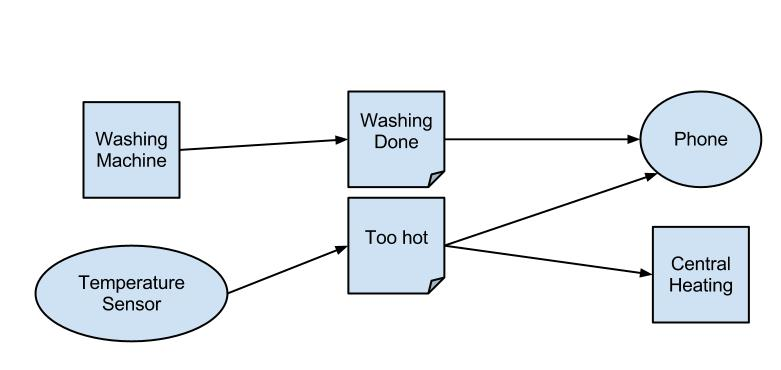
\includegraphics[scale=0.4]{JMS-IoT.jpg}
		\captionof{figure}{JMS Publish - Subscribe modelling IoT}
\end{figure}


Whilst JMS provides a well fitted framework, it does however come at a cost due to the runtime environment of Java and the additional overhead of having to run a separate server to glue the publishers and subscribers together. Whilst currently running the Java runtime on these constrained devices may not be possible, with the current pace of innovation, especially in optimisation of the Java runtime, and Moore's Law giving devices more power for the same cost and form factor every 18 months, it won't be long before it's really possible to have it running on the constrained devices of tomorrow. But until then, other alternatives and perhaps more suited tools, libraries and frameworks should be engineered starting at the lowest common denominator rather than shoe-horning large scale systems to fit constrained devices.


\begin{comment}
A fully featured pub sub system as well as point to point
pubs and subs don't know about each other but interact through Topics
Topics emulate the concept of a service very well i.e. Topic = bedroom light, living room thermostat. where subscribers can subscribe to events published to their topic

Great for large, high power machines.
Not so great on small, low power devices
JVM can be scaled down to lower power devices but still poses overhead to system.
\end{comment}
% subsection java_jms (end)

\newpage


\subsection{xAP} % (fold)
\label{sub:xap}

In the early 2000's, as an attempt to bring together a variety of technologies developed and used for Home Automation, an open source group decided to create a protocol to bridge the differences and create a unifying platform.\cite{xAP}

xAP, eXtensible Automation Protocol is designed to be a minimalist, elegant and easy to implement protocol with very basic requirements for what hardware, operating system, network and language that can run it.  
The primary implementation is based on UDP/IP with a distributed architecture where no central controller co-ordinates the network. Instead, each device either transmits or listens for data on a broadcast channel. Their core justification for this is that the network becomes fault tolerant and can withstand devices disappearing off the network for one reason or another without having a detrimental effect on the whole network.

In this design there are two key classes of devices, senders and receivers, of which a device can be either or both. 
The receiver simply attaches to the network and listens for any incoming packets, it then chooses which ones are relevant to it and processes them.
The sender attaches to the network and broadcasts packets with payloads containing data relating to its service i.e. sensor data, incoming caller ID, etc. These packets only contain enough information to uniquely identify the source and the payload it wishes to send. There is no constraint on whether or not the packet must have a destination.

This design feature makes it very simple for new devices to attach to the network and start interacting without having to go through the process of setting up connections to other devices. It also makes it very easy to implement certain types of devices like loggers or informational displays which can collect data from all senders with relative ease. However, this also creates a huge strain on the devices attached to the network which all have to receive and process any transmitted data, especially for those devices with limited resources. This becomes an increasing problem as more and more connected devices invade the home, from which the network will very quickly deteriorate as the volume of traffic being broadcast increases.

The protocol also defines a set schema for how packets should be formatted so that all devices can interoperate correctly. The schema covers both the header and the payload format, of which is almost entirely text-based, resembling albeit pre-dating JSON, with the main intention of being human readable. Whilst so, this does come at the cost of not only increasing the size of the packet considerably with redundant text, but also the complexity in parsing the data with its varying delimiters. 

After the protocol's initial inception it has had limited success, even whilst it has been continuously developed over the years, it has done so in the shadows and not in an explicitly open and collaborative way, with no central repository for code collaboration/review and no single developer's forum for discussion. % POST LINK TO YAHOO FORUMS ETC

\begin{comment}
Core Idea is to build a distributed fault tolerant IoT protocol.
total broadcasting protocol, every device just beams out its own services and any device on the network can read and interpret the data.
Can be very inefficient for devices on battery(constant barrage) and doesn't scale well with 10's, 100's, 1000's of devices.
Designed to be hardware and link agnostic and to co-exist with other protocols. Basic implementation over UDP without any care for reliability AT ALL.

Purpose is that devices can hop on and off the network without breaking/severing the entire network.

Nice concepts and goals
BUT fails to deliver a system which can scale and do things efficiently
\end{comment}
% subsection xap (end)

\subsection{OpenWSN} % (fold)
\label{sub:owsn_berkeley}
Currently being developed at the University of California, Berkeley, the Open Wireless Sensor Network project is collection of open-source implementations of protocol stacks designed against to-be-finalised ``Internet of Things'' standards, for a range of different software and hardware platforms.

%TO BE CONTINUED

% subsection owsn_berkeley (end)


\subsection{Remote Procedure Call - RPC} % (fold)
\label{sub:rpc}

% subsection rpc (end)

\subsection{Developing systems} % (fold)
\label{sub:developing_systems}

\subsubsection{Smart things} % (fold)
\label{ssub:smart_things}
Up and coming platform building upon Arduino as well as other technology to create an open eco-system of ``Things''. All things tie into a hub which is accessed through an online portal.


% subsubsection smart_things (end)

\subsubsection{Qualcomm} % (fold)
\label{ssub:qualcomm}
2013 CES Discussed bringing mobile platform hardware to IOT, but still creating a single device with internet as hub mainly 
% subsubsection qualcomm (end)
% subsection developing_systems (end)
% section existing_systems_protocols (end)



% chapter background (end)
%==============================================================================


%==============================================================================

\chapter{Requirements gathering} % (fold)
\label{cha:requirments_gathering}

% Requirements of the hardware independent design
 
% Looking at xAP, JMS, what's wrong, how can that be resolved
% what are typical use cases/ types of devices

As discussed in the previous chapter, many different platforms and protocols exist to create an ``Internet of Things'' and most take very different approaches. The rest of this section will discuss the requirements for developing a new system based on creating an ``Internet of Things'', as well as highlight several drawbacks of some the previously mentioned systems and explain how such problems can be resolved with this new approach.

Due to the nature of the target hardware platforms, constrained devices such as Arduino and TelosB, heavyweight approaches become infeasible i.e, Java \& JMS. Therefore an extremely lightweight and scalable protocol, both in terms of the protocol data unit (pdu) and the complexity in processing and managing the runtime, is a primary requirement.

Secondary to this, because of the often unstructured and ad-hoc design of a typical ``Internet of Things'' network, building a centralised system i.e, a nameserver for device search, is an un-natural fit with the network. A single failure in the server could bring the entire network down, whilst all other devices are fully operational and no way to communicate with each other.
Instead, creating a distributed system which gives all devices the power and control to communicate with each other, relieves the network of a single point of failure and can help spread the load across the network. % ADD SOMETHING TO DO WITH DISCOVERY

Taking into consideration the typical types of devices connected to the ``Internet of Things'', three general classifications of devices can be discerned; a sensor, an actuator and a controller. Sensors, anything from a temperature sensor to an open door sensor, provide a continuous service to other devices in the form of real-time data, usually from the outside world. Similarly, actuators also provide a service to other devices in the form of an interaction with the outside world, such as a speaker, light switch or thermostat. Lastly, controllers are devices which orchestrate the ``Things'' in the network, forming relationships between devices and creating useful interactions between the digital and real world i.e, connecting to both a door sensor and a light switch, when the door opens the light turns on. Whilst there are these distinct classifications, it is often the case that one class of device could overlap with another i.e, a light switch can both sense, its state, and provide an action, turn on or off.




%Heavy weight Java
%Centralised

%XAP wasteful, doesn't scale
%not easy to parse
%Some request response
%Simple to implement, simple to extend, MULTICAST, UNICAST, 
%Joining devices together rather than lone wolves connecting, cheapening links








% section problems_encountered (end)
% chapter requirments_gathering (end)
%==============================================================================


%==============================================================================


\chapter{Design} % (fold)
\label{cha:design}

% Design of system independent of hardware implementation.

\section{Protocol Design} % (fold)
\label{sec:protocol_design}
Minimal protocol, only ack required/critical data to save on transmissions.
Use some broadcasting for acquiring sensors/actuators
Provide enough guarantees for a useful and reliable system which can scale
Provide a distributed and fault tolerant way to find, collect data and control devices from
Protocol design based around several state machines. 

\subsection{Message passing} % (fold)
\label{sub:message_passing}

% subsection message_passing (end)
\subsection{States} % (fold)
\label{sub:states}
Derived states from message passing diagram blah blah.

\subsubsection{Controller} % (fold)
\label{ssub:controller}

% subsubsection controller (end)
\subsubsection{Sensor} % (fold)
\label{ssub:sensor}

% subsubsection sensor (end)
\subsubsection{Actuator} % (fold)
\label{ssub:actuator}

% subsubsection actuator (end)

% subsection states (end)


\subsection{Protocol Data Unit} % (fold)
\label{sub:protocol_data_unit}
Focus was put on reducing the pdu to as small a size as possible so to reduce the workload on both recieving/transmitting the data as well as parsing it.
% subsection protocol_data_unit (end)

\subsection{Payload Formats} % (fold)
\label{sub:payload_formats}

\subsubsection{Query} % (fold)
\label{ssub:query}
		
% subsubsection query (end)

\subsubsection{Query Response} % (fold)
\label{ssub:query_response}

% subsubsection query_response (end)

\subsubsection{Connect} % (fold)
\label{ssub:connect}

% subsubsection connect (end)

\subsubsection{Connect ACK} % (fold)
\label{ssub:connect_ack}

% subsubsection connect_ack (end)

\subsubsection{Response} % (fold)
\label{ssub:response}

% subsubsection response (end)

\subsubsection{Ping} % (fold)
\label{ssub:ping}

% subsubsection ping (end)

\subsubsection{Ping ACK} % (fold)
\label{ssub:ping_ack}

% subsubsection ping_ack (end)

\subsubsection{Disconnect} % (fold)
\label{ssub:disconnect}

% subsubsection disconnect (end)

\subsubsection{Disconnect ACK} % (fold)
\label{ssub:disconnect_ack}

% subsubsection disconnect_ack (end)
% subsection payload_formats (end)


% section protocol_design (end)




% chapter design (end)
%==============================================================================


%==============================================================================


\chapter{Implementation} % (fold)
\label{cha:implementation}
% Describe the problems encountered in the implementation of arduino and then contiki

\section{Arduino} % (fold)
\label{sec:arduino}
Whilst given its user base and ideology makes it a great platform to build for, the immediate lack of compatible hardware and lack of certain expectations leaves it difficult to develop an efficient implementation of the system.

No interrupts
% section arduino (end)


\section{Telos B Motes and Contiki} % (fold)
\label{sec:contiki}
Great, well defined and established hardware.
Contiki is a comprehensive and well devised OS which provides a simple learning curve for a C programmer with only some event magic thrown in.

\subsection{Choosing the transport layer:IP4 vs IPv6 vs Rime} % (fold)
\label{sub:ip4_vs_ipv6_vs_rime}

% subsection ip4_vs_ipv6_vs_rime (end)

\subsection{Problems Encountered} % (fold)
\label{sub:problems_encountered}

\subsubsection{Event driven system} % (fold)
\label{sub:event_driven_system}

% subsubsection event_driven_system (end)

\subsubsection{IPv4 Broadcast support} % (fold)
\label{sub:ipv4_broadcast_support}

% subsubsection ipv4_broadcast_support (end)
% subsection problems_encountered (end)

% section contiki (end)
% chapter implementation (end)
%==============================================================================


%==============================================================================


\chapter{Evaluation} % (fold)
\label{cha:evaluation}

% chapter evaluation (end)

%==============================================================================


%==============================================================================


\chapter{Conclusion} % (fold)
\label{cha:conclusion}


% chapter conclusion (end)
%==============================================================================


%%%%%%%%%%%%%%%%
%              %
%  APPENDICES  %
%              %
%%%%%%%%%%%%%%%%
\begin{appendices}


\end{appendices}

%%%%%%%%%%%%%%%%%%%%
%   BIBLIOGRAPHY   %
%%%%%%%%%%%%%%%%%%%%

\bibliographystyle{plain}
\bibliography{bib}

\end{document}
